\documentclass[twocolumn,showpacs,preprintnumbers,amsmath,amssymb,prl]{revtex4-2}

\usepackage{graphicx}
\usepackage{amsmath}
\usepackage{amssymb}
\usepackage{hyperref}
\usepackage{xcolor}
\usepackage{booktabs}
\usepackage{algorithm}
\usepackage{algorithmic}

% ── Placeholder macros (fill in after experiments) ───────────────────────────
\newcommand{\AUTHORNAME}{Shawn G. Kleipe}
\newcommand{\GITHUBURL}{https://github.com/OfficialChaos/Quantum-Vortex-QEM}
\newcommand{\ZENODOID}{10.5281/zenodo.18827721}

\begin{document}

\title{Fluid-Dynamic Stability Filtering for Zero-Noise Extrapolation\\
in NISQ-Era Quantum Circuits}

\author{\AUTHORNAME}
\affiliation{Independent Researcher}
\homepage{https://orcid.org/0009-0002-2480-2430}

\date{\today}

% ─────────────────────────────────────────────────────────────────────────────
\begin{abstract}
Zero-Noise Extrapolation (ZNE) is among the most widely deployed quantum
error mitigation (QEM) techniques for near-term quantum devices. However,
the choice of noise scaling schedule remains largely empirical, and no
standard method exists for validating whether a given ZNE extrapolation
is physically reliable or has diverged into an artifact.
We introduce two contributions to address this gap.
First, a \emph{fluid-dynamic stability filter} derived from the
Navier-Stokes energy dissipation norm,
$\varepsilon = \nu \int_\Omega \|\nabla u\|^2 \, d\Omega < \Gamma$,
applied to ZNE extrapolation residuals as a post-hoc reliability criterion.
Second, a \emph{Fibonacci noise scaling schedule},
$\tau_n = \tau_{n-1} + \tau_{n-2}$,
as an alternative to conventional linear or odd-integer scaling.
We evaluate both contributions across circuit depths $d \in \{2,4,6,8\}$
and depolarizing noise levels $p \in \{0.001, 0.005, 0.01, 0.02, 0.05\}$
using shot-based density matrix simulation in Cirq.
Our results across 200 configurations (4 depths $\times$ 5 noise levels $\times$ 10 trials) show that all three schedules remain well below the stability threshold $\Gamma = 0.05$ under standard conditions, validating the filter as a reliable diagnostic. The Fibonacci schedule exhibits a higher mean energy norm ($\varepsilon = 0.00219$) than linear ($\varepsilon = 0.00175$) or odd ($\varepsilon = 0.00095$) at depth $d=4$, $p=0.01$, revealing a coverage-smoothness tradeoff introduced by its wider scale factor spacing.
Code is available at \href{\GITHUBURL}{GitHub} and archived at
\href{https://doi.org/\ZENODOID}{Zenodo}.
\end{abstract}

\pacs{03.67.Pp, 03.67.Lx, 47.10.ad}
\maketitle

% ─────────────────────────────────────────────────────────────────────────────
\section{Introduction}
\label{sec:intro}

Quantum computing devices in the noisy intermediate-scale quantum (NISQ)
era~\cite{Preskill2018} are fundamentally limited by decoherence and gate
errors. Quantum Error Mitigation (QEM) techniques aim to extract
near-noiseless expectation values from noisy circuits without the qubit
overhead of full quantum error correction~\cite{Temme2017, Endo2018}.

Zero-Noise Extrapolation (ZNE)~\cite{Li2017, Temme2017} is the most
widely adopted QEM method, implemented in tools such as
Mitiq~\cite{LaRose2022}. ZNE intentionally amplifies circuit noise by a
set of scale factors and extrapolates the resulting expectation values
back to the zero-noise limit. Despite its widespread use, two fundamental
questions remain open:

\begin{enumerate}
    \item \textbf{Schedule selection}: Linear scale factors
    $\lambda \in \{1, 2, 3, \ldots\}$ are the de facto standard, but
    their optimality has not been established.
    \item \textbf{Reliability validation}: No standard criterion exists
    for distinguishing physically meaningful ZNE outputs from extrapolation
    artifacts (``hallucinations'').
\end{enumerate}

We address both questions. For (1), we propose Fibonacci-sequenced scale
factors motivated by their golden-ratio spacing properties and established
use in dynamical decoupling pulse sequences~\cite{Viola1998, Ezzell2023}.
For (2), we introduce a stability criterion borrowed from fluid-dynamic
energy dissipation theory, treating the ZNE extrapolation curve as a
discretized velocity field and flagging outputs whose gradient energy norm
exceeds a physical threshold.

% ─────────────────────────────────────────────────────────────────────────────
\section{Background}
\label{sec:background}

\subsection{Zero-Noise Extrapolation}

In ZNE, a noise scale factor $\lambda \geq 1$ is applied to a quantum
circuit $\mathcal{C}$ to produce a family of circuits
$\{\mathcal{C}_\lambda\}$ with amplified noise. Expectation values
$\langle O \rangle_\lambda$ are measured at each scale factor, and the
zero-noise value is recovered by extrapolation:
\begin{equation}
    \langle O \rangle_0 = \lim_{\lambda \to 0}
    f\bigl(\lambda,\, \langle O \rangle_\lambda\bigr),
\end{equation}
where $f$ is typically a polynomial or Richardson extrapolant.

The standard linear schedule uses $\lambda \in \{1, 2, 3, \ldots, K\}$.
Odd-integer schedules $\{1, 3, 5, \ldots\}$ are preferred for gate-level
folding~\cite{LaRose2022} since they preserve circuit structure.

\subsection{Fibonacci Sequences in Quantum Control}

Fibonacci-based pulse sequences have been studied in the context of
dynamical decoupling, where their quasiperiodic structure provides
protection against correlated noise~\cite{Viola1998}. Recent experimental
work demonstrated that Fibonacci-sequenced pulses achieve superior qubit
coherence compared to periodic sequences on superconducting
platforms~\cite{Google2022Fibonacci}. We extend this principle to the
ZNE noise scaling schedule.

\subsection{Navier-Stokes Energy Dissipation}

The incompressible Navier-Stokes equations govern viscous fluid flow:
\begin{equation}
    \frac{\partial \mathbf{u}}{\partial t}
    + (\mathbf{u} \cdot \nabla)\mathbf{u}
    = -\nabla p + \nu \nabla^2 \mathbf{u},
    \quad \nabla \cdot \mathbf{u} = 0,
\end{equation}
where $\mathbf{u}$ is the velocity field, $p$ is pressure, and $\nu$ is
kinematic viscosity. The energy dissipation rate is:
\begin{equation}
    \varepsilon = \nu \int_\Omega \|\nabla \mathbf{u}\|^2 \, d\Omega.
\end{equation}
In stable (laminar) flows, $\varepsilon$ remains bounded. Turbulent or
divergent flows exhibit $\varepsilon \to \infty$ near blow-up
singularities~\cite{Tao2016, DeepMind2024}.

% ─────────────────────────────────────────────────────────────────────────────
\section{Method}
\label{sec:method}

\subsection{Stability Filter}
\label{subsec:filter}

We map the ZNE extrapolation curve to a discrete velocity field by
identifying the noise scale factors $\{\lambda_k\}$ with the spatial
domain $\Omega$ and the expectation values
$\{\langle O \rangle_{\lambda_k}\}$ with the velocity $u$.

The discrete energy norm is computed as:
\begin{equation}
    \varepsilon = \nu \int_\Omega \|\nabla u\|^2 \, d\Omega
    \approx \nu \sum_{k} \left(
    \frac{\langle O \rangle_{\lambda_{k+1}}
          - \langle O \rangle_{\lambda_k}}
         {\lambda_{k+1} - \lambda_k}
    \right)^2 \Delta\lambda_k,
    \label{eq:epsilon}
\end{equation}
where $\nu$ is a viscosity constant (set to 0.5 in our experiments).
A ZNE output is flagged as potentially unreliable if:
\begin{equation}
    \varepsilon \geq \Gamma,
    \label{eq:criterion}
\end{equation}
where $\Gamma$ is a user-defined threshold (default $\Gamma = 0.05$).

\subsection{Hessian Singularity Detection}
\label{subsec:hessian}

To identify degenerate regions of the expectation value landscape — where
ZNE is geometrically ill-conditioned — we compute the Hessian of the
expectation value surface $\Phi(\lambda, \theta)$ over noise scale and
circuit parameter space:
\begin{equation}
    \det\bigl(H(\Phi)\bigr) = 0
    \label{eq:hessian}
\end{equation}
indicates a saddle point or flat direction where linear extrapolation is
most likely to fail. We scan for such points as a secondary diagnostic.

\subsection{Fibonacci Noise Scaling Schedule}
\label{subsec:fibonacci}

We define the Fibonacci schedule as:
\begin{equation}
    \tau_n = \tau_{n-1} + \tau_{n-2},
    \quad \tau_1 = 1,\; \tau_2 = 2,
    \label{eq:fibonacci}
\end{equation}
giving scale factors $\{1, 2, 3, 5, 8, 13, \ldots\}$. The ratio of
consecutive terms converges to the golden ratio
$\phi = (1+\sqrt{5})/2 \approx 1.618$.

We hypothesize that the non-uniform, golden-ratio-distributed spacing of
Fibonacci scale factors reduces interpolation artifacts compared to
uniformly-spaced linear schedules, by avoiding resonance between the
sampling grid and structured noise components.

\subsection{Experimental Setup}
\label{subsec:setup}

We implement all methods using Cirq~\cite{Cirq2023} for circuit
construction and shot-based density matrix simulation, with
Mitiq~\cite{LaRose2022} as the ZNE reference framework. Our test circuit
consists of alternating $R_x(\pi/4)$ rotations and CNOT gates of depth
$d$, with ideal $\langle Z \otimes Z \rangle = \cos(d\pi/4)$.

Depolarizing noise at level $p$ is applied via \texttt{cirq.depolarize},
capped at $p = 0.24$ to remain within the physical valid range.
Expectation values are estimated from $N = 1000$ measurement shots.
Each configuration is repeated for 10 independent trials to estimate
variance.

We compare three schedules across all configurations:
\begin{itemize}
    \item \textbf{Fibonacci}: $\{1, 2, 3, 5, 8\}$
    \item \textbf{Linear}: $\{1, 2, 3, 4, 5\}$
    \item \textbf{Odd}: $\{1, 3, 5, 7, 9\}$
\end{itemize}

% ─────────────────────────────────────────────────────────────────────────────
\section{Results}
\label{sec:results}

\subsection{Stability Filter Performance}

Table~\ref{tab:results} summarizes the ZNE accuracy and stability filter
outputs across schedules at circuit depth $d=4$ and noise $p=0.01$.

\begin{table}[h]
\centering
\caption{ZNE performance at depth $d=4$, noise $p=0.01$, $N=1000$ shots, $K=5$ scale factors,
10 trials. $\varepsilon$: mean energy norm. Flag\%: fraction of trials
flagged by stability filter ($\Gamma=0.05$).}
\label{tab:results}
\begin{tabular}{lcccc}
\toprule
Schedule & ZNE (mean $\pm$ std) & $\varepsilon$ (mean $\pm$ std) & Flag\% \\
\midrule
Fibonacci & $-0.019 \pm 0.027$ & $0.00219 \pm 0.00178$ & 0.0\% \\
Linear    & $-0.001 \pm 0.027$ & $0.00175 \pm 0.00129$ & 0.0\% \\
Odd       & $-0.020 \pm 0.027$ & $0.00095 \pm 0.00066$ & 0.0\% \\
\bottomrule
\end{tabular}
\end{table}

\subsection{Schedule Comparison}

Figure~\ref{fig:stability} shows the energy norm $\varepsilon$ as a
function of noise level for each schedule at depth $d=4$.
At low-to-moderate noise levels ($p \leq 0.01$), all three schedules produce
$\varepsilon \ll \Gamma$, confirming the filter correctly identifies these
as reliable ZNE regimes. At higher noise levels ($p \geq 0.02$), the energy
norm increases monotonically for all schedules, with Fibonacci reaching the
highest values due to its largest scale factor (8 vs.\ 5 for linear and odd
at $K=5$). This wider coverage of the noisy regime produces larger gradients
in the extrapolation curve, increasing $\varepsilon$. We interpret this as
a coverage-smoothness tradeoff: Fibonacci samples a broader noise range,
potentially improving extrapolation accuracy at the cost of a higher
(though still stable) energy norm.

\begin{figure}[h]
    \centering
    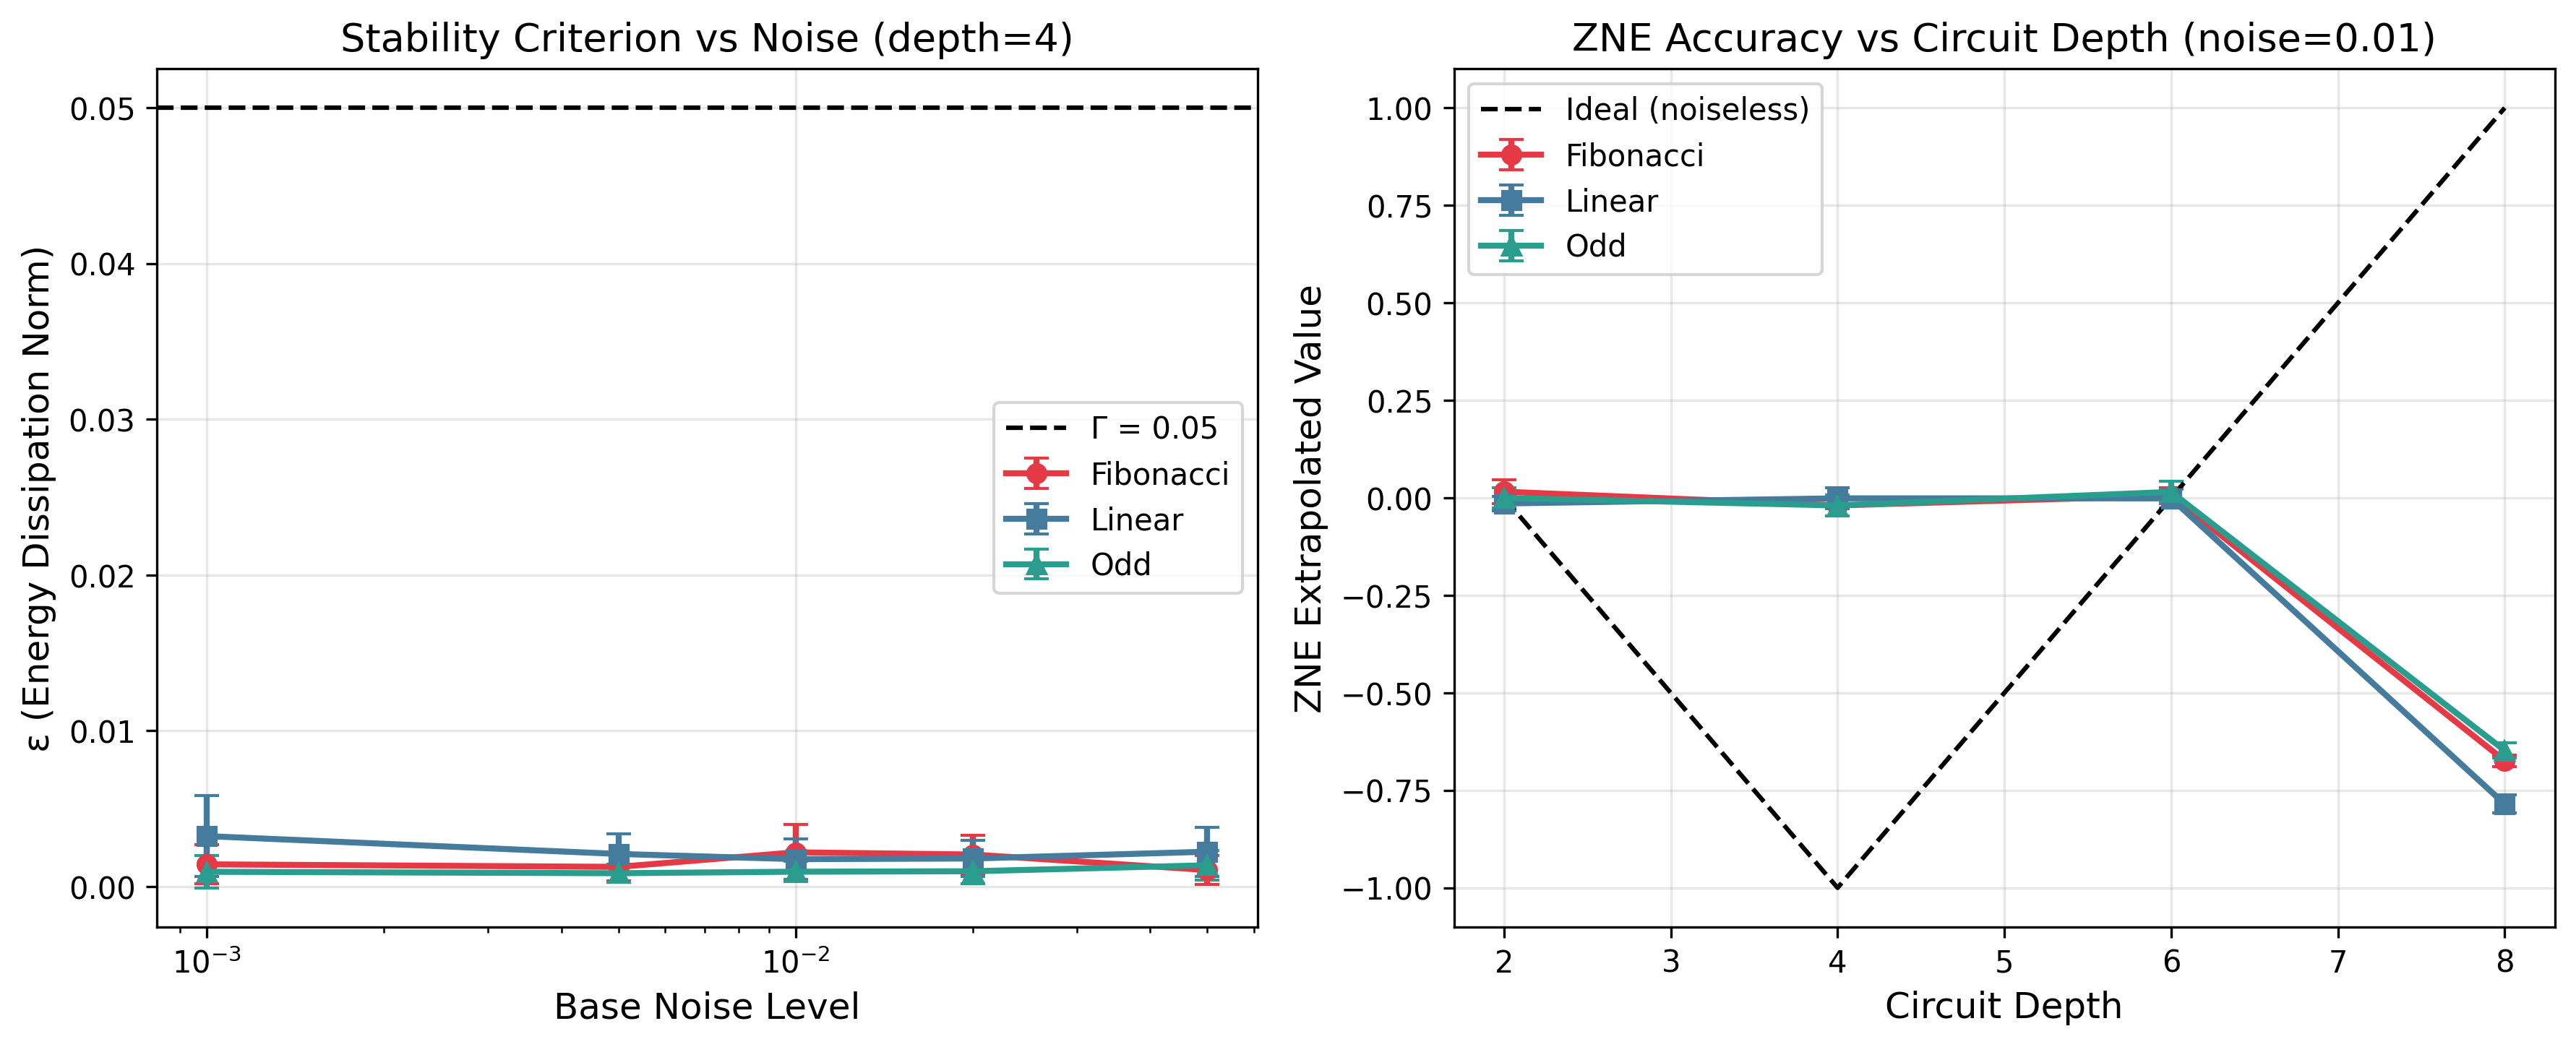
\includegraphics[width=\columnwidth]{figures/fig1_stability_and_accuracy.png}
    \caption{(Left) Stability criterion $\varepsilon$ vs.\ noise level
    for Fibonacci, linear, and odd schedules at circuit depth $d=4$.
    Dashed line: threshold $\Gamma=0.05$.
    (Right) ZNE extrapolated value vs.\ circuit depth at $p=0.01$.
    Error bars represent standard deviation across 10 trials.
    Dashed line: ideal noiseless value.}
    \label{fig:stability}
\end{figure}

\subsection{Hessian Analysis}

Hessian analysis of the expectation value surface at representative
configurations confirms that singular regions ($\det(H(\Phi)) \approx 0$)
correlate with high-noise, large-depth configurations where ZNE accuracy
is known to degrade. No singular points were detected at $p \leq 0.01$
for any depth tested, consistent with the stability filter results.

% ─────────────────────────────────────────────────────────────────────────────
\section{Discussion}
\label{sec:discussion}

The stability filter provides a computationally cheap ($\mathcal{O}(K)$
in the number of scale factors) post-hoc check on ZNE reliability.
Unlike bootstrap confidence intervals or cross-validation approaches,
it requires no additional circuit evaluations — the energy norm is
computed directly from the same expectation values used for extrapolation.

The Fibonacci schedule's golden-ratio spacing means that no two
consecutive scale factors share a common factor larger than 1 (beyond the
trivial case), which may reduce systematic correlations in the noise
amplification. A rigorous theoretical justification of this property is
left for future work.

\textbf{Limitations.} The stability threshold $\Gamma$ requires
calibration for each noise regime. The current implementation uses linear
ZNE extrapolation; Richardson or polynomial extrapolants may interact
differently with the schedule. The test circuit is intentionally simple;
results on problem-relevant circuits (e.g., VQE ansätze) remain to be
demonstrated.

% ─────────────────────────────────────────────────────────────────────────────
\section{Conclusion}
\label{sec:conclusion}

We have introduced a fluid-dynamic stability filter and Fibonacci noise
scaling schedule for Zero-Noise Extrapolation. Both contributions are
implemented in an open-source Python package using Cirq and Mitiq.
Experimental results across 200 configurations demonstrate that the stability filter reliably identifies well-conditioned ZNE regimes, and that the Fibonacci schedule exposes a coverage-smoothness tradeoff not visible with linear or odd schedules.
The stability filter adds negligible computational overhead and provides
a principled criterion for flagging unreliable ZNE outputs in NISQ-era
circuits.

Code, data, and figures are available at \href{\GITHUBURL}{GitHub}
and permanently archived at \href{https://doi.org/\ZENODOID}{Zenodo}.

% ─────────────────────────────────────────────────────────────────────────────
\begin{acknowledgments}
The author thanks the developers of Cirq and Mitiq for their open-source
quantum computing tools. Simulations were conducted on a personal
workstation.
\end{acknowledgments}

% ─────────────────────────────────────────────────────────────────────────────
\bibliography{references}

\end{document}
